\documentclass{article}
\usepackage{fullpage}
\usepackage{graphicx}
\title{\begin{Huge}\textbf{Software Report}\end{Huge}\\
        \textbf{Random Music Player}\\
\textbf{AI1110}:Probability And Random Variables}

\author{\textbf{RAJIV CHAUDHARY}\\
\textbf{AI22BTECH11021}}

\date{}
\begin{document}
\maketitle

\section{Aim}
This report aims to document the implementation of a code that playsrandom song from music playlist using python.The code utilizes Random and Pydub library for shuffle the code and plays song in a random way.
\section {Library}
\begin{enumerate}
        \item \textbf{Random} it will shuffte the playlist of song.
        \item \textbf{Pydub} pydub library allows to load the song and play song.
\end{enumerate}
\section{Implementation}
\begin{enumerate}
        \item first import random and pydub library.
        \item From pydub import Audiosegment and from pydub.playback import play.
        \item create list of songs.
        \item In name write full address of song.
        \item Now apply for loop in list.
        \item Using Audiosegment load the song.
        \item Using play to play the song.
        \item After playing the song,a message is printed that if you want to continue or quit.
        \item If you choose continue,it will restart the playlist.
        \item If you choose quit,it will stop.
\end{enumerate}
\section{Conclusion}
In this way, a music playlist can be generated using Python playing random songs.
\begin{figure}[h]
        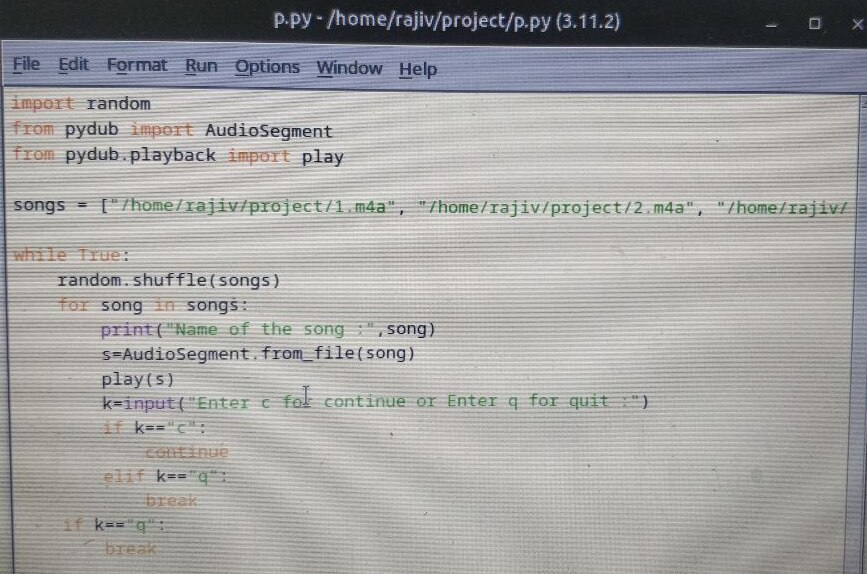
\includegraphics[width=\linewidth]{1.jpg}     
        \caption{code}
        \label{output}
\end{figure}
\begin{figure}[h]
        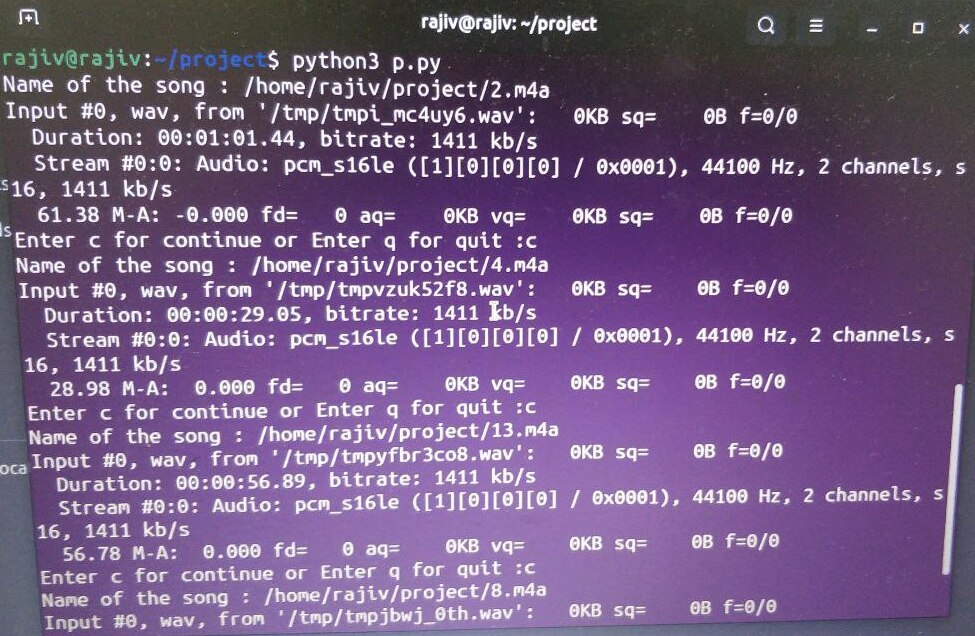
\includegraphics[width=\linewidth]{2.jpg}     
        \caption{output}
        \label{output}
\end{figure}
\end{document}

